\documentclass[11pt,journal,a4paper]{IEEEtran}

\usepackage[T1]{fontenc}
\usepackage{amsmath,amssymb}
\usepackage{graphicx}
\usepackage{booktabs}
\usepackage{multirow}
\usepackage{tikz}
\usetikzlibrary{arrows.meta}
\usepackage{cite}
\usepackage[hidelinks]{hyperref}

\graphicspath{{../figures/}}
\markboth{DA5453 Project Report}{DA5453 Project Report}

\newtheorem{proposition}{Proposition}
\newcommand{\Aoo}{A_{\mathrm{oil,oil}}}
\newcommand{\xb}{\bar{x}}
\newcommand{\E}{\mathbb{E}}

\begin{document}

\title{Taste Heterogeneity and the Linear Context Logit: Re-examining the Sushi Context Effect}

\author{Madhav~Tadepalli,~EE23B040, and Advik~Kabra,~CS23B004%
\thanks{DA5453 Learning from Human Preferences, IIT Madras. Course project on Tomlinson and Benson,
``Learning Interpretable Feature Context Effects in Discrete Choice'' (KDD 2021).}}

\maketitle

\begin{abstract}
The linear context logit (LCL) of Tomlinson and Benson lets the mean features of a choice set change a
chooser's preferences, and tests each such context effect with a likelihood-ratio test. On the sushi data,
where menus are random, the paper finds that people avoid oily sushi more when the menu is oilier
($A_{\mathrm{oil,oil}}=-0.27$, $p=1.6\times10^{-6}$) and suggests that the effect may be causal. We test whether
the same pattern can arise because people differ in how much they like oily food. A second-order expansion
shows that a population with taste variance $s^2$ behaves like a single chooser whose oiliness weight falls by
$s^2$ times the menu's weighted mean oiliness, which an LCL reads as a negative self-effect. In simulations on
the real sushi menus with no context effect, a normal spread of tastes or two segments of people reproduce the
paper's estimate and its significance for $s\approx0.8$--$1.0$. The same test run inside a random-coefficient
logit flags 0--1\% of these datasets and still detects a true effect of the paper's size in 91\% of cases. On the
real data the fitted taste spread is 0.45. A parametric bootstrap attributes about a third of the effect to it,
and inside heterogeneity models the effect falls to $-0.21$ with $p\approx10^{-3}$. Using each respondent's
second and third ranked choices, the effect is $-0.06$ ($p=0.23$) and $+0.02$ ($p=0.73$), with a test that we
show detects the paper's effect size in 94--100\% of simulated datasets. A first-pick effect of about $-0.15$
($p\approx0.02$) remains.
\end{abstract}

\begin{IEEEkeywords}
Discrete choice, context effects, linear context logit, mixed logit, preference heterogeneity.
\end{IEEEkeywords}

%======================================================================
\section{Introduction}

\IEEEPARstart{M}{ost} discrete choice models assume independence of irrelevant alternatives (IIA): the
relative odds of two items do not depend on what else is offered. Behavioural work finds many violations,
called context effects. Tomlinson and Benson~\cite{tb21} propose the linear context logit (LCL), in which the
mean features of the choice set shift the chooser's preference vector through a matrix $A$. The model keeps
a concave log-likelihood, and each entry $A_{pq}$ has a direct reading (how feature $q$ on the menu changes
the weight on feature $p$) and a likelihood-ratio test (LRT).

The paper's main interpretable result is on the sushi data~\cite{kamishima03}. Each of 5,000 respondents ranks
a random set of 10 sushi drawn from 100. The most significant effect is the oiliness self-effect,
$\Aoo=-0.20$ in the full model and $-0.27$ when fitted alone (LRT 23, $p=1.5\times10^{-6}$). Because the menus
are random, the authors suggest that it may be a causal effect, in which an oily menu makes oily sushi less
appealing.

Random menus remove choice-set confounding~\cite{tub21}, where menus depend on the chooser. They do not
remove taste heterogeneity, where different people have different coefficients. If some people like oily
sushi and others avoid it, an oily menu spreads the first group's choices over many oily items while the
second group concentrates on the few light ones. Each oily item is then chosen less often on an oily menu,
although no individual's preferences depend on the menu. The paper compares LCL with a mixed logit as a
separate model, but it does not test the oiliness effect inside a model that allows tastes to vary.

Our question is whether LCL can tell a context effect apart from taste heterogeneity, and whether the sushi
oiliness effect remains once heterogeneity is modelled.

We think this is worth asking for two reasons. First, what makes LCL attractive is that each entry of $A$ can
be read and tested on its own. If heterogeneity alone produces significant entries, then a significant entry
tells us that the data are not MNL, but not that the menu changes anyone's preferences, and causal readings
like the one above need a different test. Second, the question can actually be answered. A context effect
acts on every choice a person makes from a menu, while a taste difference stays with the person. So the two
explanations make different predictions as soon as we observe the same person choosing more than once, and
the sushi data, which record a full ranking for every respondent, let us do that.

Our approach has four parts. We first reproduce the paper's numbers. We then work out what heterogeneity looks
like to an LCL, using a second-order expansion. Next, we simulate choices on the real sushi menus from ground
truths that we control, including two kinds of heterogeneity without any context effect, and compare the
paper's test with the same test run inside a heterogeneity model. Finally, we return to the real data.

Our contributions are:
\begin{itemize}
\item An exact reproduction of the paper's sushi results.
\item A second-order expansion showing why taste heterogeneity appears to an LCL as a negative self-effect,
      checked numerically on the real menus.
\item A simulation study on the real sushi menus with two kinds of heterogeneity (a continuous normal spread
      and discrete segments), comparing the paper's test with the same test inside heterogeneity models.
\item A re-analysis of the real data: tests inside heterogeneity models, a parametric bootstrap, and a panel
      analysis that uses the full rankings the paper discards, with a simulation check of that test.
\end{itemize}

\subsection{Related Work}

That averaging over people can create context effects is known outside machine learning. Hutchinson,
Kamakura and Lynch~\cite{hkl00} showed that context (``reversal'') effects in choice experiments can arise from
pooling segments of consumers that do not show the effect separately. Liew, Howe and Little~\cite{lhl16}
analysed participants in classic context-effect experiments individually and found that few showed the
effects seen in the averaged data. In econometrics, the distinction between true and spurious state
dependence~\cite{heckman81} has the same structure, and is resolved with repeated observations of the same
person. Mixed logit can approximate any random utility model~\cite{mcfadden00}, and the similarity effect of
Tversky~\cite{tversky72} is the standard example of a pattern it produces without context effects~\cite{train09}.
Marketing models include explicit context-effect terms next to context-free part-worths so that both are
estimated together~\cite{rvb11}.

In machine learning, LCL follows the context-dependent random utility model of Seshadri et
al.~\cite{spu19}. Seshadri and Ugander~\cite{su20} show that testing IIA in general needs a number of samples
exponential in the number of alternatives. Tomlinson, Ugander and Benson~\cite{tub21} show that choice sets
that depend on the chooser bias preference estimates. In the LCL paper, the comparison that allows for
heterogeneity on sushi (DLCL against mixed logit) gives LRT 59, $p=0.0089$, which does not meet the paper's
$p<0.001$ threshold, and LCL does not improve held-out prediction on sushi ($p=0.31$). The oiliness effect
itself is tested only against a plain MNL. We did not find work that tests LCL's individual effects inside a
heterogeneity model.

%======================================================================
\section{Methods}

\subsection{Models}

A chooser picks item $i$ from a set $C$, and item $i$ has features $x_i\in\mathbb{R}^d$. The multinomial
logit (MNL) has $\Pr(i\mid C)\propto\exp(\theta^\top x_i)$. The LCL~\cite{tb21} uses a preference vector that
depends on the set:
\begin{equation}
\Pr(i\mid C)\propto\exp\big((\theta+A\xb_C)^\top x_i\big),\qquad \xb_C=\frac{1}{|C|}\sum_{j\in C}x_j.
\label{eq:lcl}
\end{equation}
An entry $A_{pq}$ is tested with an LRT against MNL in which only that entry is free (the paper's constrained
LCL). We use two models of taste heterogeneity in which every individual is an MNL chooser~\cite{train09}:
\begin{itemize}
\item random coefficients (RC): $\theta_n=\theta+\eta_n$, $\eta_n\sim\mathcal{N}(0,\mathrm{diag}(\sigma^2))$
      on selected features;
\item latent classes (LC): $\theta_n=\theta+\delta_c$ with probability $\pi_c$, $c=1,\dots,K$.
\end{itemize}
Both can be combined with $A$. The test of $\Aoo$ inside RC or LC is a one-degree-of-freedom LRT between the
heterogeneity model with and without that entry. When a person makes several choices, $\eta_n$ is shared
across them (a panel model).

\subsection{Heterogeneity Seen Through an LCL}

To see why heterogeneity can look like a context effect, consider the simplest case. Person $n$ has
$\theta_n=\mu+\eta_ne_k$, so that everyone agrees except on feature $k$, with $\E\eta_n=0$ and
$\mathrm{Var}\,\eta_n=s^2$. For a set $C$, let $p_j$ be the MNL probabilities at the average taste $\mu$, and
let $m_C=\sum_jp_jx_{jk}$ and $v_C=\sum_jp_j(x_{jk}-m_C)^2$ be the weighted mean and variance of feature $k$
in the set.

\begin{proposition}\label{prop:expansion}
The population choice probabilities $P_i=\E_\eta\Pr_{\mu+\eta e_k}(i\mid C)$ satisfy
\begin{equation}
\log P_i=\mu^\top x_i+\frac{s^2}{2}x_{ik}^2-s^2m_C\,x_{ik}-Z_C+O(\E|\eta|^3),
\label{eq:expansion}
\end{equation}
where $Z_C$ is the same for every item in $C$.
\end{proposition}

\begin{IEEEproof}
Let $f(\eta)$ be the log-probability of item $i$ at taste $\mu+\eta e_k$. Differentiating the log-softmax
gives $f'(0)=x_{ik}-m_C$ and $f''(0)=-v_C$, so
$P_i=p_i\big(1+\tfrac{s^2}{2}[(x_{ik}-m_C)^2-v_C]\big)+O(\E|\eta|^3)$. Taking logs and expanding the square,
the terms $m_C^2$ and $v_C$ do not depend on $i$ and go into $Z_C$.
\end{IEEEproof}

In words, a population of ordinary logit choosers who disagree about feature $k$ behaves, to second order,
like one chooser with two extra terms. The first is a curvature term in $x_{ik}$. The second is a coefficient
on feature $k$ that falls as the menu's weighted mean of $k$ rises, which is exactly the shape of a negative
LCL self-effect. In sushi, a regression of $m_C$ on the plain set mean $\xb_{C,\mathrm{oil}}$ has slope
$\beta=1.16$, so an LCL fitted to such data should report $A_{kk}\approx-\beta s^2$. Two further points follow.
The LCL has no $x_{ik}^2$ term, so part of the curvature is absorbed elsewhere and the fitted value is smaller
in size; adding a squared term removes this attenuation and makes the spurious effect larger rather than
removing it. And since only the variance $s^2$ enters at this order, a normal spread and a population of
segments should give the same effect when $s$ is small.

There is also a limit to what heterogeneity can do. Any mixture of logits is a random utility model, and
every random utility model satisfies regularity: adding an item to a menu never raises the probability of an
item that was already there~\cite{bm60}. Heterogeneity can therefore produce negative self-effects of the
similarity type, but never an effect that breaks regularity, such as the attraction effect~\cite{hpp82}.

\subsection{Pipeline of the Simulation Study}

Fig.~\ref{fig:pipeline} shows the simulation design. We keep the 5,000 real sushi menus and their item
features, and simulate only the choices, from a ground truth that we choose. The base tastes are the MNL fit to
sushi. The ground truths are: no effect (MNL); a true effect $\Aoo=-0.266$ with identical people; a normal
spread of the oiliness coefficient with standard deviation $s$; two segments with equal shares, or with
shares 20/80, whose oiliness coefficients have variance $s^2$; and a smaller true effect ($-0.15$) together with
a normal spread ($s=0.75$). Each simulated dataset is fitted with MNL, the full LCL, the one-entry LCL, and
three models with and without $\Aoo$: a random coefficient on oiliness (RC), two latent classes on oiliness
(LC2), and an MNL with a squared oiliness term (SQ). We use the paper's threshold $p<0.001$ and 100
replicates per setting.

\begin{figure}[!t]
\centering
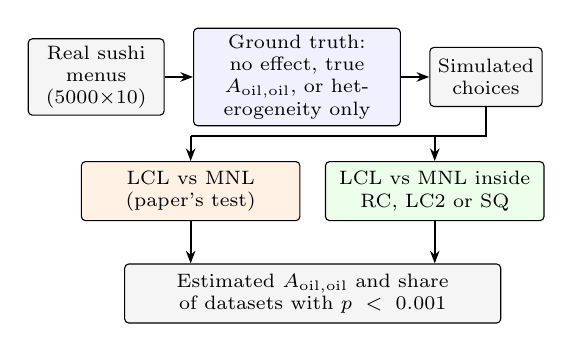
\begin{tikzpicture}[
  box/.style={draw,rounded corners=1.5pt,align=center,font=\scriptsize,inner sep=2.5pt,minimum height=0.75cm},
  arr/.style={-{Stealth[length=1.6mm]},thick}]
\node[box,fill=gray!8,text width=1.55cm] (menus) at (0,0) {Real sushi menus (5000$\times$10)};
\node[box,fill=blue!6,text width=2.45cm] (truth) at (2.55,0) {Ground truth: no effect, true $\Aoo$, or heterogeneity only};
\node[box,fill=gray!8,text width=1.25cm] (sim) at (4.95,0) {Simulated choices};
\node[box,fill=orange!10,text width=2.6cm] (paper) at (1.2,-1.45) {LCL vs MNL\\(paper's test)};
\node[box,fill=green!8,text width=2.6cm] (ours) at (4.3,-1.45) {LCL vs MNL inside RC, LC2 or SQ};
\node[box,fill=gray!8,text width=4.6cm] (out) at (2.75,-2.75) {Estimated $\Aoo$ and share of datasets with $p<0.001$};
\draw[arr] (menus) -- (truth);
\draw[arr] (truth) -- (sim);
\draw[thick] (sim.south) -- (4.95,-0.75) -- (1.2,-0.75);
\draw[arr] (1.2,-0.75) -- (paper.north);
\draw[arr] (4.3,-0.75) -- (ours.north);
\draw[arr] (paper.south) -- (paper.south |- out.north);
\draw[arr] (ours.south) -- (ours.south |- out.north);
\end{tikzpicture}
\caption{Simulation design. Menus and item features are the real sushi ones; only the choices are
simulated.}
\label{fig:pipeline}
\end{figure}

\subsection{Dataset}

The sushi data~\cite{kamishima03} has 5,000 respondents, each ranking 10 of 100 sushi from most to least
preferred. Following the authors' code, we take the top-ranked item as the
choice and use six features, standardised over all item occurrences: is maki, is seafood, oiliness,
popularity, price and availability. Oiliness is coded from 0 (oily) to 4 (light); the self-effect $\Aoo$ does
not depend on the direction of the coding. The data also include gender, age group and whether the respondent
grew up in eastern or western Japan.

For the panel analysis we treat a ranking as successive choices (the rank-ordered logit~\cite{beggs81}): the
best of 10, then the best of the remaining 9, and so on. With the top $k$ ranks each respondent gives $k$
choices, made from menus whose mean features change from stage to stage.

\subsection{Implementation Details}

All models are written in PyTorch as one class with optional $A$ entries, squared terms, demographic
interactions, random coefficients and latent classes. We fit by exact maximum likelihood with L-BFGS in
double precision and without regularisation, so that the LRTs are not affected by a penalty. RC likelihoods
use 200 scrambled Sobol draws per person (100 in panel models). Latent-class models use several random
restarts. Nested models are fitted starting from each other's optimum, which keeps every LRT statistic
non-negative. We only test entries of $A$; LRTs for variance parameters lie on the boundary of the parameter
space and are not used. The simulation study took about four hours on 8 CPU cores, and the bootstrap and panel
checks about one hour together.

%======================================================================
\section{Results}

\subsection{Reproduction}

Table~\ref{tab:repro} compares our fits with the paper. The numbers agree to the reported precision. Two other
single effects are significant at $p<0.001$: price on price ($-0.18$) and price on oiliness ($+0.18$).

\begin{table}[!t]
\caption{Reproduction of the paper's sushi results (LRT: all 36 entries of $A$)}
\label{tab:repro}
\centering\footnotesize
\setlength{\tabcolsep}{3pt}
\begin{tabular}{lcccc}
\toprule
 & MNL NLL & LCL NLL & LRT & $\Aoo$ full / alone \\
\midrule
Paper~\cite{tb21} & 9821 & 9773 & 97 & $-0.20$ / $-0.26$ \\
Ours & 9821.4 & 9772.7 & 97.3 & $-0.204$ / $-0.266$ \\
\bottomrule
\end{tabular}
\end{table}

\subsection{Check of the Expansion}

We simulated 100,000 choices on the real menus (each menu used 20 times) with heterogeneity in oiliness only,
and fitted an MNL with the two regressors of \eqref{eq:expansion}, $x_{ik}^2$ and $m_Cx_{ik}$, added
(Table~\ref{tab:oracle}). For $s=0.25$ the fitted coefficients are close to $s^2/2$ and $-s^2$ for all three
taste distributions. For larger $s$ the signs stay correct but the sizes are smaller than predicted, and the
three distributions start to differ, which is the expected effect of third-order terms.

\begin{table}[!t]
\caption{Fitted coefficients of the two terms in (2), over three taste distributions with variance $s^2$}
\label{tab:oracle}
\centering\footnotesize
\setlength{\tabcolsep}{3.5pt}
\begin{tabular}{ccccc}
\toprule
 & \multicolumn{2}{c}{$x_{ik}^2$} & \multicolumn{2}{c}{$m_C\,x_{ik}$} \\
\cmidrule(lr){2-3}\cmidrule(lr){4-5}
$s$ & theory & fitted & theory & fitted \\
\midrule
0.25 & 0.031 & 0.022 to 0.031 & $-0.062$ & $-0.060$ to $-0.051$ \\
0.50 & 0.125 & 0.100 to 0.121 & $-0.250$ & $-0.203$ to $-0.183$ \\
1.00 & 0.500 & 0.250 to 0.318 & $-1.000$ & $-0.511$ to $-0.385$ \\
\bottomrule
\end{tabular}
\end{table}

\subsection{Simulation Study}

Fig.~\ref{fig:spurious} shows the mean $\Aoo$ reported by the one-entry LCL when no one in the population has
a context effect. The estimate grows with the taste spread and reaches the paper's $-0.27$ at
$s\approx0.8$--$1.0$. This is the central result of the simulation: the effect the paper reports is what
LCL finds in a population of context-free choosers whose tastes differ by about one standard deviation. The
three taste distributions agree at $s=0.5$, as the proposition predicts, and segments give a larger effect than
a normal spread with the same variance at larger $s$. In our first pilot, which used synthetic Gaussian
item features instead of the sushi items, the same spread gave a much smaller effect ($-0.06$ at $s=1$), so the
size of the bias depends on the menu design.

\begin{figure}[!t]
\centering
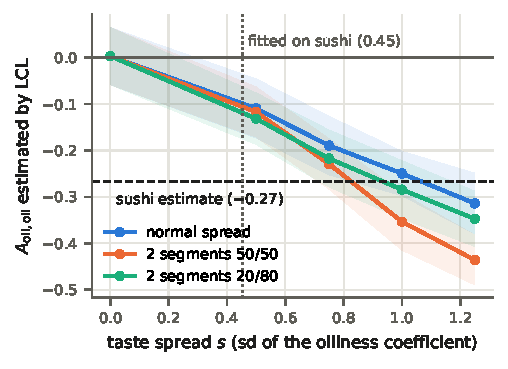
\includegraphics[width=\columnwidth]{ieee_spurious.pdf}
\caption{Mean $\Aoo$ estimated by the one-entry LCL on simulated data with no context effect, against the
spread $s$ of the oiliness coefficient (shading: $\pm1$ sd over 100 replicates). The dotted line is the
spread fitted on the real data.}
\label{fig:spurious}
\end{figure}

Fig.~\ref{fig:rejections} and Table~\ref{tab:sim} give the rejection rates. The paper's test flags an effect in
57--78\% of datasets at $s=0.75$ and in 92--99\% at $s=1$. The same test inside RC or LC2 flags 0--1\% of these
datasets at every $s$, and detects the true effect in 91\% (RC) and 88\% (LC2) of datasets, against 94\% for the
paper's test. So modelling heterogeneity removes the false positives while costing very little power, and
this holds whether the heterogeneity is continuous or comes from segments. When a true effect of $-0.15$ is combined with heterogeneity, RC estimates $-0.14$ while the
paper's test reports $-0.30$; at this smaller effect size RC detects it in only 10\% of datasets. A normal RC
fitted to data from two segments leaves a small negative estimate at large $s$ ($-0.08$ to $-0.11$) but rarely
a significant one. The squared term does not help: inside SQ the false-positive rate is 45--100\%, as the
expansion predicts. Finally, at equal parameter counts, RC fits better than the one-entry LCL in all
heterogeneity datasets and in none of the true-effect datasets.

\begin{figure*}[!t]
\centering
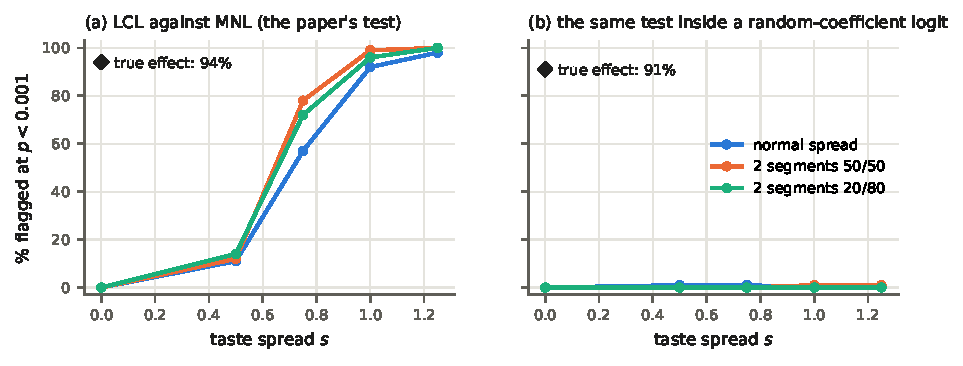
\includegraphics[width=\textwidth]{ieee_rejections.pdf}
\caption{Share of simulated datasets in which $\Aoo$ is significant at $p<0.001$. (a) The paper's test. (b) The
same test inside a random-coefficient logit. Diamonds: datasets with a true effect of the paper's size and no
heterogeneity.}
\label{fig:rejections}
\end{figure*}

\begin{table*}[!t]
\caption{Simulation results (100 replicates per row; rates vary by about $\pm5$--10 points).
$^{*}$Significant and at least as negative as the paper's $-0.266$}
\label{tab:sim}
\centering\footnotesize
\setlength{\tabcolsep}{4.5pt}
\begin{tabular}{llcccccccc}
\toprule
 & & \multicolumn{4}{c}{LCL against MNL} & \multicolumn{4}{c}{test of $\Aoo$ inside \dots}\\
\cmidrule(lr){3-6}\cmidrule(lr){7-10}
Ground truth & $s$ & mean $\Aoo$ & 36-df & single & as paper$^{*}$ & RC: mean $\Aoo$ & RC & LC2 & SQ\\
\midrule
no effect & 0 & $+0.00$ & 0\% & 0\% & 0\% & $+0.01$ & 0\% & 0\% & 0\%\\
true effect $-0.27$ & 0 & $-0.26$ & 21\% & 94\% & 44\% & $-0.25$ & 91\% & 88\% & 91\%\\
effect $-0.15$ + normal spread & 0.75 & $-0.30$ & 75\% & 98\% & 72\% & $-0.14$ & 10\% & 6\% & 100\%\\
\midrule
\multirow{4}{*}{normal spread} & 0.50 & $-0.11$ & 2\% & 11\% & 1\% & $-0.00$ & 1\% & 0\% & 45\%\\
 & 0.75 & $-0.19$ & 33\% & 57\% & 11\% & $-0.00$ & 1\% & 1\% & 98\%\\
 & 1.00 & $-0.25$ & 88\% & 92\% & 39\% & $+0.02$ & 0\% & 0\% & 100\%\\
 & 1.25 & $-0.31$ & 100\% & 98\% & 77\% & $+0.01$ & 0\% & 0\% & 100\%\\
\midrule
\multirow{4}{*}{two segments, 50/50} & 0.50 & $-0.12$ & 3\% & 12\% & 0\% & $-0.00$ & 0\% & 0\% & 57\%\\
 & 0.75 & $-0.23$ & 61\% & 78\% & 25\% & $-0.02$ & 0\% & 0\% & 100\%\\
 & 1.00 & $-0.35$ & 100\% & 99\% & 94\% & $-0.08$ & 1\% & 0\% & 100\%\\
 & 1.25 & $-0.44$ & 100\% & 100\% & 100\% & $-0.11$ & 1\% & 0\% & 100\%\\
\midrule
\multirow{4}{*}{two segments, 20/80} & 0.50 & $-0.13$ & 4\% & 14\% & 2\% & $-0.01$ & 0\% & 0\% & 76\%\\
 & 0.75 & $-0.22$ & 60\% & 72\% & 26\% & $+0.00$ & 0\% & 0\% & 100\%\\
 & 1.00 & $-0.28$ & 99\% & 96\% & 60\% & $+0.04$ & 0\% & 0\% & 100\%\\
 & 1.25 & $-0.35$ & 100\% & 100\% & 93\% & $+0.05$ & 0\% & 0\% & 100\%\\
\bottomrule
\end{tabular}
\end{table*}

\subsection{Heterogeneity Models on the Sushi Data}

Table~\ref{tab:real} tests $\Aoo$ inside several heterogeneity models fitted to the paper's data. Letting the
oiliness coefficient vary adds one parameter and improves the log-likelihood by 13.9 over MNL. It also fits
better than the one-entry LCL ($-9809.8$), which has the same number of parameters. Inside every heterogeneity
model the effect falls to about $-0.21$ and its $p$-value rises to about $10^{-3}$, the paper's threshold.
Demographics change tastes (women prefer lighter sushi) but do not change $\Aoo$. Inside RC on all features,
price on price goes from $p=4\times10^{-4}$ to $0.014$ and price on oiliness from $6\times10^{-4}$ to $0.039$.
The test of all 36 entries of $A$ remains significant (LRT 97 to 78, $p=7\times10^{-5}$).

\begin{table}[!t]
\caption{Test of $\Aoo$ inside heterogeneity models, sushi data with one choice per person}
\label{tab:real}
\centering\footnotesize
\setlength{\tabcolsep}{3pt}
\begin{tabular}{lccc}
\toprule
Base model & log-lik. & $\Aoo$ & LRT ($p$) \\
\midrule
MNL (paper) & $-9821.4$ & $-0.266$ & 23.1 ($1.6\times10^{-6}$) \\
MNL + squared oiliness & $-9820.7$ & $-0.296$ & 27.5 ($1.5\times10^{-7}$) \\
RC, oiliness (sd 0.45) & $-9807.5$ & $-0.214$ & 10.9 ($9.4\times10^{-4}$) \\
RC, all features & $-9804.3$ & $-0.220$ & 10.7 ($1.0\times10^{-3}$) \\
2 classes, oiliness & $-9807.1$ & $-0.214$ & 10.9 ($9.6\times10^{-4}$) \\
2 classes, all features & $-9799.0$ & $-0.207$ & 9.8 ($1.7\times10^{-3}$) \\
Demographics & $-9757.5$ & $-0.265$ & 22.7 ($1.9\times10^{-6}$) \\
Demographics + RC, all & $-9741.0$ & $-0.216$ & 10.4 ($1.2\times10^{-3}$) \\
\bottomrule
\end{tabular}
\end{table}

\subsection{Parametric Bootstrap}

We fitted heterogeneity models without context effects to the sushi data, simulated 200 datasets from each
on the real menus, and repeated the paper's analysis (Fig.~\ref{fig:boot}). With the fitted spread of 0.45, the
mean estimate is $-0.09$, about a third of the observed $-0.27$. The effect is significant at $p<0.001$ in 3--6\%
of these datasets (12\% for a three-class model) and as negative as $-0.266$ in at most 0.5\%. None reaches the
paper's 36-entry LRT of 97. With one choice per person, the fitted heterogeneity explains part of the effect
but not all of it.

\begin{figure}[!t]
\centering
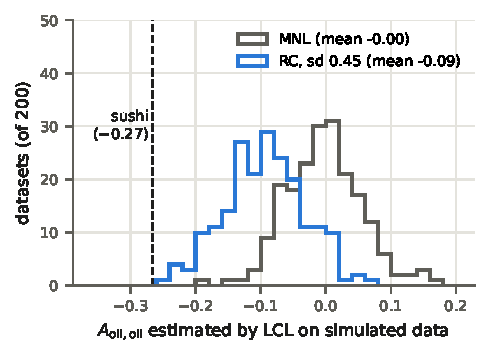
\includegraphics[width=\columnwidth]{ieee_bootstrap.pdf}
\caption{Parametric bootstrap. $\Aoo$ estimated by the one-entry LCL on 200 datasets simulated from MNL and
from a random-coefficient logit fitted to sushi. Models with two classes or with all features heterogeneous
give almost the same distribution (mean $-0.09$).}
\label{fig:boot}
\end{figure}

\subsection{Panel Analysis with the Full Rankings}

With one choice per person, a person's taste and the menu are hard to separate. Using the top $k$ ranks gives
$k$ choices per person with a shared taste $\eta_n$ and a menu mean that changes between stages.
Table~\ref{tab:panel} shows the result. Inside a panel RC on all features, the effect is $-0.06$ ($p=0.23$)
with $k=2$ and $+0.02$ ($p=0.73$) with $k=3$, while an LCL without heterogeneity becomes more significant as
$k$ grows.

\begin{table}[!t]
\caption{Sushi data with the top $k$ ranked choices per person}
\label{tab:panel}
\centering\footnotesize
\setlength{\tabcolsep}{3pt}
\begin{tabular}{ccc}
\toprule
$k$ & LCL: $\Aoo$ ($p$) & panel RC + $\Aoo$: $\Aoo$ ($p$) \\
\midrule
1 & $-0.266$ ($1.6\times10^{-6}$) & $-0.220$ ($1.0\times10^{-3}$) \\
2 & $-0.243$ ($1.6\times10^{-10}$) & $-0.064$ ($0.23$) \\
3 & $-0.228$ ($5.7\times10^{-14}$) & $+0.015$ ($0.73$) \\
\bottomrule
\end{tabular}
\end{table}

To check that the panel test could have found the effect, we simulated 50 ranking datasets per ground truth on
the real menus, choosing one stage at a time so that a true LCL effect acts on the remaining items at each
stage, with tastes from the sushi panel fit (Table~\ref{tab:panelcheck}). With heterogeneity and no context
effect, the panel test flags no dataset, while the LCL without heterogeneity flags 78\% ($k=2$) and 100\%
($k=3$). With a true effect of $-0.266$, the panel test detects it in 94--100\% of datasets. In ranking data
the later menus depend on each person's earlier picks, so heterogeneity becomes choice-set
confounding~\cite{tub21}, which explains the growing bias of the plain LCL.

\begin{table}[!t]
\caption{Simulation check of the panel test (50 datasets per row; flagged: $p<0.001$)}
\label{tab:panelcheck}
\centering\footnotesize
\setlength{\tabcolsep}{2.5pt}
\begin{tabular}{lccccc}
\toprule
 & & \multicolumn{2}{c}{LCL} & \multicolumn{2}{c}{panel RC + $\Aoo$} \\
\cmidrule(lr){3-4}\cmidrule(lr){5-6}
Ground truth & $k$ & $\Aoo$ & flagged & $\Aoo$ & flagged \\
\midrule
Heterogeneity only & 2 & $-0.16$ & 78\% & $+0.00$ & 0\% \\
 & 3 & $-0.22$ & 100\% & $+0.01$ & 0\% \\
Heterogeneity + effect & 2 & $-0.38$ & 100\% & $-0.25$ & 94\% \\
 & 3 & $-0.43$ & 100\% & $-0.26$ & 100\% \\
Effect only & 2 & $-0.26$ & 100\% & $-0.26$ & 100\% \\
 & 3 & $-0.27$ & 100\% & $-0.26$ & 100\% \\
\bottomrule
\end{tabular}
\end{table}

\subsection{First Pick and Later Picks}

We then allowed separate self-effects for the first pick, made from the full menu, and for later picks.
Without heterogeneity both stages show the effect ($-0.23$ and $-0.25$ with $k=2$, both $p<10^{-4}$). Inside
the panel RC, the later picks show no effect ($+0.04$, $p=0.61$ with $k=2$; $+0.09$, $p=0.06$ with $k=3$),
while the first pick keeps one of $-0.16$ ($p=0.017$) with $k=2$ and $-0.14$ ($p=0.034$) with $k=3$. This could
be a reaction to the full menu at the first choice, or heterogeneity that a diagonal normal model does not
capture, such as correlated tastes. Our data do not separate the two.

\subsection{Observation}

Putting the pieces together, the sushi evidence weakens at each step. With one choice per person, the paper's
test gives $p=1.6\times10^{-6}$. Allowing tastes to vary moves this to about $10^{-3}$, and the bootstrap says
that the heterogeneity we can measure accounts for about a third of the estimate. Once each person's taste is
pinned down by their second and third choices, the effect is gone at the later picks and only a smaller
first-pick effect is left, at $p\approx0.02$. The simulations make clear why the first step is misleading: a
significant negative self-effect is exactly what an LCL reports for a population whose tastes differ, even
when the menus are random.

The regularity argument limits the scope of this result. Heterogeneity can only produce effects that are
consistent with a random utility model, so effects that imply regularity violations, or positive self-effects
such as the paper's ``truck on truck'' effect in car-alt, need another explanation; for car-alt the authors
found that menus were tailored to respondents. We also do not claim that sushi has no context effects: the test
of all 36 entries remains significant after heterogeneity is modelled.

Several limitations apply. The rank-ordered model assumes the same utility at every rank, while lower ranks
are known to be noisier~\cite{hr87}; with $k=5$ the panel estimate becomes $+0.12$ ($p=9\times10^{-4}$), so we
use $k\le3$, which we checked by simulation. Our heterogeneity models are diagonal normal or have at most three
classes, and correlated tastes were not tried. The simulations use 100 replicates per setting (50 in the
panel check), so rates are uncertain by about $\pm5$--10 points. The expansion is accurate only for small $s$.

%======================================================================
\section{Conclusion}

We reproduced the sushi results of the linear context logit and tested whether its oiliness self-effect can
be explained by differences in taste between people. Theory and simulations on the real menus show that taste
heterogeneity, with no context effect, produces a negative self-effect of the paper's size and significance,
and that testing the effect inside a random-coefficient or latent-class model keeps the false-positive rate
at the nominal level with little loss of power. On the real data, the fitted heterogeneity explains about a
third of the effect with one choice per person. With two or three ranked choices per person, the effect is
not distinguishable from zero at later picks, and a first-pick effect of about $-0.15$ remains at
$p\approx0.02$. We conclude that the paper's causal reading of the oiliness effect is not supported once taste
heterogeneity is modelled. The practical lesson is simple: an LCL effect should be tested inside a
heterogeneity model, using repeated choices per person when the data have them. This keeps what we like about
LCL, its interpretable and convex structure, and each of our fits took only seconds. Future work is to apply the same tests to the paper's other
datasets and to try richer heterogeneity models for the remaining first-pick effect.

\appendices
\section{Sources of Code and Data}
\begin{itemize}
\item Data: sushi preference data \texttt{sushi3-2016.zip}~\cite{kamishima03} from the author's website
      (\url{https://www.kamishima.net/sushi/}); it may not be redistributed, so it is not in our repository.
\item Reference code: the feature preprocessing follows the authors' repository
      (\url{https://github.com/tomlinsonk/feature-context-effects}).
\item Our code: \texttt{lcl\_heterogeneity/src} (data loading, models, reproduction, expansion check,
      simulation study, real-data analysis, bootstrap, panel check and figures), with all outputs in
      \texttt{lcl\_heterogeneity/results}.
\item Libraries: PyTorch, NumPy, SciPy, pandas, Matplotlib.
\end{itemize}

\section*{Acknowledgment}
We used Claude (Anthropic), through the Claude Code assistant, to help write the analysis scripts, run the
experiments and draft this report.

\begin{thebibliography}{99}
\bibitem{tb21} K.~Tomlinson and A.~R.~Benson, ``Learning interpretable feature context effects in discrete
  choice,'' in \emph{Proc. ACM SIGKDD Conf. Knowledge Discovery and Data Mining (KDD)}, 2021.
\bibitem{kamishima03} T.~Kamishima, ``Nantonac collaborative filtering: Recommendation based on order
  responses,'' in \emph{Proc. ACM SIGKDD Conf. Knowledge Discovery and Data Mining (KDD)}, 2003,
  pp.~583--588.
\bibitem{tub21} K.~Tomlinson, J.~Ugander, and A.~R.~Benson, ``Choice set confounding in discrete choice,'' in
  \emph{Proc. ACM SIGKDD Conf. Knowledge Discovery and Data Mining (KDD)}, 2021.
\bibitem{hkl00} J.~W.~Hutchinson, W.~A.~Kamakura, and J.~G.~Lynch, ``Unobserved heterogeneity as an
  alternative explanation for `reversal' effects in behavioral research,'' \emph{J. Consumer Research},
  vol.~27, no.~3, pp.~324--344, 2000.
\bibitem{lhl16} S.~X.~Liew, P.~D.~L.~Howe, and D.~R.~Little, ``The appropriacy of averaging in the study of
  context effects,'' \emph{Psychonomic Bulletin \& Review}, vol.~23, no.~5, pp.~1639--1646, 2016.
\bibitem{heckman81} J.~J.~Heckman, ``Heterogeneity and state dependence,'' in \emph{Studies in Labor
  Markets}, S.~Rosen, Ed. Chicago, IL, USA: Univ. Chicago Press, 1981, pp.~91--140.
\bibitem{mcfadden00} D.~McFadden and K.~Train, ``Mixed MNL models for discrete response,'' \emph{J. Applied
  Econometrics}, vol.~15, no.~5, pp.~447--470, 2000.
\bibitem{tversky72} A.~Tversky, ``Elimination by aspects: A theory of choice,'' \emph{Psychological Review},
  vol.~79, no.~4, pp.~281--299, 1972.
\bibitem{train09} K.~Train, \emph{Discrete Choice Methods with Simulation}, 2nd~ed. Cambridge, U.K.:
  Cambridge Univ. Press, 2009.
\bibitem{rvb11} R.~P.~Rooderkerk, H.~J.~van~Heerde, and T.~H.~A.~Bijmolt, ``Incorporating context effects into
  a choice model,'' \emph{J. Marketing Research}, vol.~48, no.~4, pp.~767--780, 2011.
\bibitem{spu19} A.~Seshadri, A.~Peysakhovich, and J.~Ugander, ``Discovering context effects from raw choice
  data,'' in \emph{Proc. Int. Conf. Machine Learning (ICML)}, 2019.
\bibitem{su20} A.~Seshadri and J.~Ugander, ``Fundamental limits of testing the independence of irrelevant
  alternatives in discrete choice,'' arXiv:2001.07042, 2020.
\bibitem{bm60} H.~D.~Block and J.~Marschak, ``Random orderings and stochastic theories of responses,'' in
  \emph{Contributions to Probability and Statistics}, I.~Olkin \emph{et~al.}, Eds. Stanford, CA, USA:
  Stanford Univ. Press, 1960, pp.~97--132.
\bibitem{hpp82} J.~Huber, J.~W.~Payne, and C.~Puto, ``Adding asymmetrically dominated alternatives: Violations
  of regularity and the similarity hypothesis,'' \emph{J. Consumer Research}, vol.~9, no.~1, pp.~90--98, 1982.
\bibitem{beggs81} S.~Beggs, S.~Cardell, and J.~Hausman, ``Assessing the potential demand for electric cars,''
  \emph{J. Econometrics}, vol.~17, no.~1, pp.~1--19, 1981.
\bibitem{hr87} J.~A.~Hausman and P.~A.~Ruud, ``Specifying and testing econometric models for rank-ordered
  data,'' \emph{J. Econometrics}, vol.~34, no.~1--2, pp.~83--104, 1987.
\end{thebibliography}

\end{document}
